%4619055 課題4
\documentclass[12pt]{jarticle}
\usepackage{TUSIreport}
\usepackage{otf}
\usepackage[dvipdfmx]{graphicx}
\usepackage{amsmath}
\usepackage{amssymb}
\usepackage{hhline}
\usepackage{fancybox,ascmac}
\usepackage{url}
\usepackage{multirow}
%%%%%%%%%%%%%%%%%%
\begin{document}
%%%%%%%%%%%%%%%%%%%%%%%%%%%%%%%%%%%%%%%%%%%%%%%%%%%%%%%%
% 表紙を出力する場合は,\提出者と\共同実験者をいれる
% \提出者{科目名}{課題名}{提出年}{提出月}{提出日}{学籍番号}{氏名}
% \共同実験者{一人目}{二人目}{..}{..}{..}{..}{..}{八人目}
%%%%%%%%%%%%%%%%%%%%%%%%%%%%%%%%%%%%%%%%%%%%%%%%%%%%%%%
\提出者{情報工学実験1}{課題4 統計学入門}
{2020}{8}{3}{4619055}{辰川力駆}

\共同実験者{}{}{}{}{}{}{}{}
\追加実験者{}{}
\表紙出力

\section{実験の目的}
\begin{itemize}
    \item[(1)] 離散分布の理解

          代表的な離散分布である二項分布を理解する。
    \item[(2)]標本平均の分布

          中心極限定理を理解する。
    \item[(3)] 連続分布の理解

          代表的な連続分布である正規分布を理解する。
\end{itemize}

\section{実験1}
二項分布を基にした実験

\subsection{目標}
離散分布の基本として二項分布の特徴を理解する。
\subsection{実験手順}
\begin{itemize}
    \item[(1)] ``赤4個、白6個の合計10個の玉が入った箱から1つ取り出して色を確認後、
          取り出した玉を箱に戻す作業を5回繰り返す。"
          というのを1回の試行として、これを30回試行して記録する。
    \item[(2)] 取り出された赤玉の回数の度数表と棒グラフをExcelで作成する。
    \item[(3)] 取り出された赤玉の個数の平均値を求める。
\end{itemize}
\subsection{実験結果}
以下に実験結果の表とグラフを示す。
また、取り出された赤玉の個数の平均値は約2.433333333となった。

\clearpage
\begin{table}
    \begin{center}
        \caption{試行における赤玉の個数}
        \begin{tabular}[h]{|c|c|c|c|c|c|c|}
            \hline
            \multirow{2}{*}{試行} & \multicolumn{5}{|c|}{回数} & \multirow{2}{*}{赤玉の個数}                    \\
            \cline{2-6}
                                  & 1                          & 2                           & 3  & 4  & 5  &   \\
            \hline
            1                     & 〇                         & 〇                          & 〇 & ×  & 〇 & 4 \\
            2                     & ×                          & 〇                          & ×  & 〇 & ×  & 2 \\
            3                     & 〇                         & ×                           & 〇 & 〇 & ×  & 3 \\
            4                     & ×                          & 〇                          & ×  & ×  & 〇 & 2 \\
            5                     & ×                          & ×                           & 〇 & 〇 & ×  & 2 \\
            6                     & 〇                         & ×                           & 〇 & ×  & ×  & 2 \\
            7                     & 〇                         & ×                           & 〇 & ×  & 〇 & 3 \\
            8                     & 〇                         & ×                           & 〇 & 〇 & 〇 & 4 \\
            9                     & ×                          & ×                           & ×  & 〇 & ×  & 1 \\
            10                    & ×                          & ×                           & 〇 & ×  & ×  & 1 \\
            11                    & ×                          & 〇                          & ×  & ×  & 〇 & 2 \\
            12                    & ×                          & 〇                          & 〇 & 〇 & ×  & 3 \\
            13                    & 〇                         & 〇                          & 〇 & 〇 & ×  & 4 \\
            14                    & 〇                         & 〇                          & ×  & 〇 & ×  & 3 \\
            15                    & 〇                         & 〇                          & 〇 & ×  & ×  & 3 \\
            16                    & 〇                         & ×                           & 〇 & 〇 & 〇 & 4 \\
            17                    & ×                          & ×                           & ×  & ×  & ×  & 0 \\
            18                    & ×                          & ×                           & ×  & 〇 & 〇 & 2 \\
            19                    & 〇                         & ×                           & ×  & 〇 & 〇 & 3 \\
            20                    & 〇                         & ×                           & 〇 & 〇 & ×  & 3 \\
            21                    & ×                          & 〇                          & 〇 & ×  & 〇 & 3 \\
            22                    & 〇                         & ×                           & ×  & ×  & ×  & 1 \\
            23                    & ×                          & ×                           & ×  & ×  & 〇 & 1 \\
            24                    & ×                          & 〇                          & 〇 & 〇 & 〇 & 4 \\
            25                    & ×                          & ×                           & 〇 & 〇 & 〇 & 3 \\
            26                    & 〇                         & ×                           & ×  & ×  & 〇 & 2 \\
            27                    & 〇                         & ×                           & 〇 & ×  & ×  & 2 \\
            28                    & 〇                         & 〇                          & ×  & 〇 & 〇 & 4 \\
            29                    & 〇                         & ×                           & ×  & ×  & ×  & 1 \\
            30                    & ×                          & ×                           & 〇 & ×  & ×  & 1 \\
            \hline
                                  & \multicolumn{5}{|c|}{平均} & 2.433333333                                    \\
            \hline
        \end{tabular}
    \end{center}
\end{table}
\clearpage

\begin{table}
    \begin{center}
        \caption{出現回数の度数表}
        \begin{tabular}[h]{|c|c|}
            \hline
            赤玉の個数 & 度数 \\
            \hline
            0          & 1    \\
            1          & 6    \\
            2          & 8    \\
            3          & 9    \\
            4          & 6    \\
            5          & 0    \\
            \hline
        \end{tabular}
    \end{center}
\end{table}
\begin{figure}[h]
    \begin{center}
        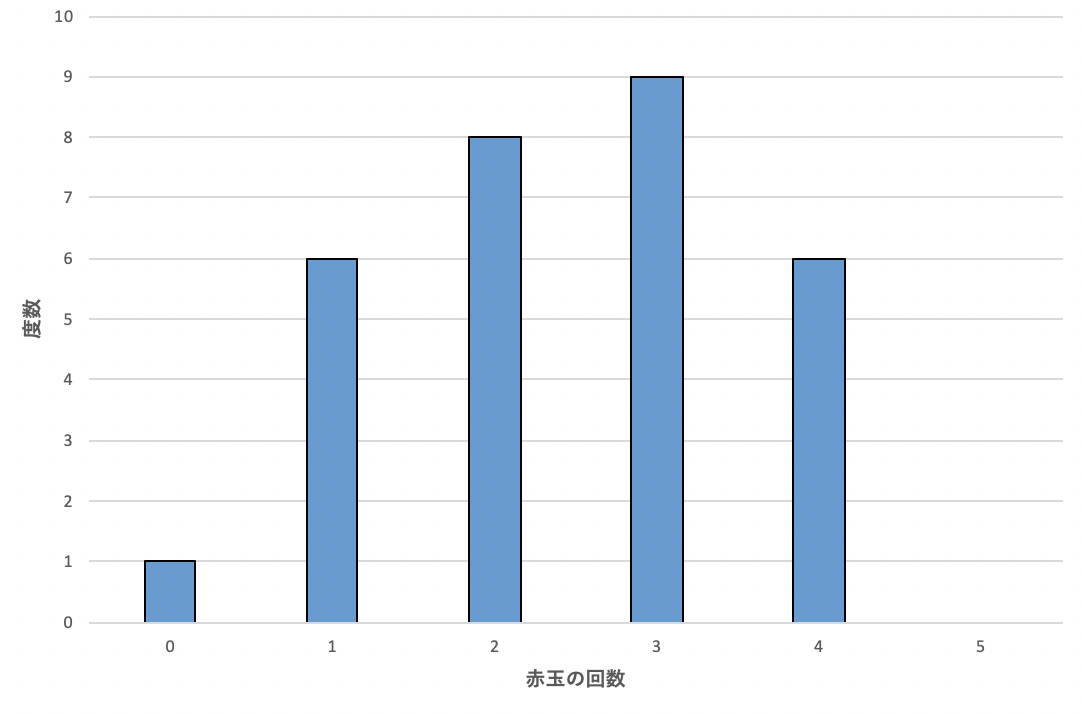
\includegraphics[scale=0.9]{kadai4_1graph1.png}
    \end{center}
    \caption{赤玉出現回数の棒グラフ}
\end{figure}
\clearpage

\subsection{レポート課題}
\subsubsection*{レポート課題1-1}
\begin{shadebox}
    実験1の結果をまとめよ。
\end{shadebox}
表 2 の度数分布表より,最頻値は 1 であり,表 1 の実験結果より,平均値は 1.83 である.中
央値は 2 である.ヒストグラムから見ると,1 の頻度が結構高いので,平均値が中央値より小
さいと考えられる.

\subsubsection*{レポート課題1-2}
\begin{shadebox}
    実験1の結果は、二項分布に従っているといえるか述べよ。
\end{shadebox}
実験1の結果は、二項分布に従っていない。


\section{実験2}
中心極限定理を基にした実験

\subsection{目標}
\begin{itemize}
    \item データを視覚的に表現する方法を理解する
    \item データの正しい要約を行う
\end{itemize}

\subsection{実験手順}
\begin{itemize}
    \item[(1)] 年収データの平均値・中央値・最頻値を求める
    \item[(2)] 年収を50万円刻みで区切ったヒストグラムを作成する
    \item[(3)] 箱ひげ図を作成する
\end{itemize}

\subsection{実験結果}
\begin{figure}[h]
    \begin{center}
        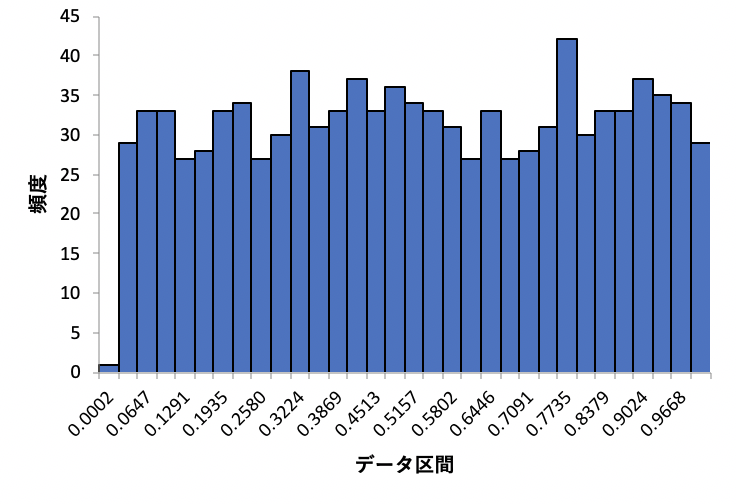
\includegraphics[scale=0.7]{kadai4_2graph1.png}
    \end{center}
    \caption{}
\end{figure}
\begin{figure}[h]
    \begin{center}
        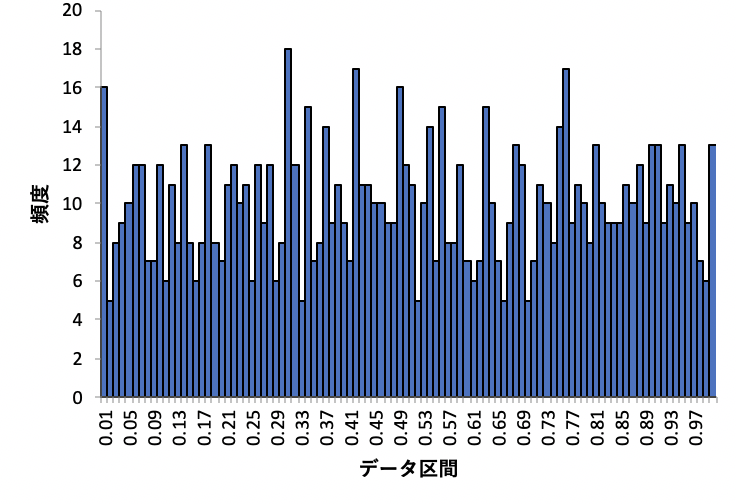
\includegraphics[scale=0.7]{kadai4_2graph2.png}
    \end{center}
    \caption{}
\end{figure}
\begin{figure}[h]
    \begin{center}
        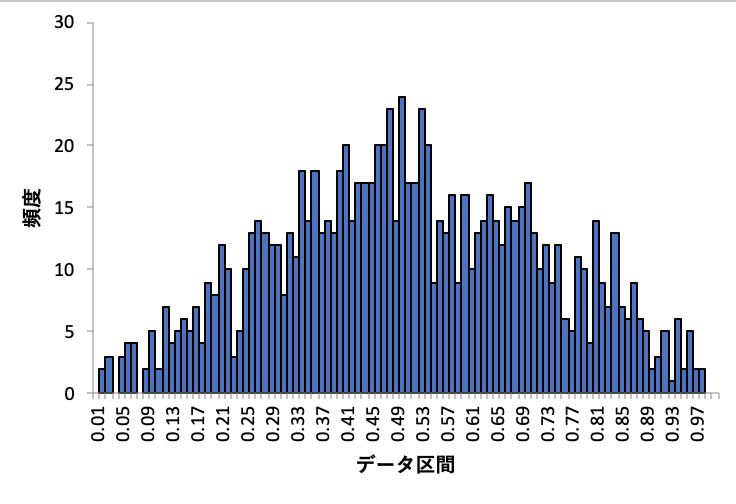
\includegraphics[scale=0.7]{kadai4_2graph3.png}
    \end{center}
    \caption{}
\end{figure}
\begin{figure}[h]
    \begin{center}
        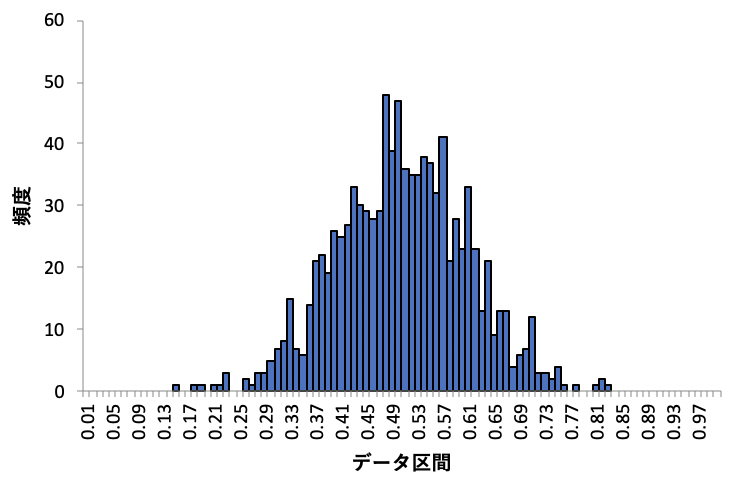
\includegraphics[scale=0.7]{kadai4_2graph4.png}
    \end{center}
    \caption{}
\end{figure}
\begin{figure}[h]
    \begin{center}
        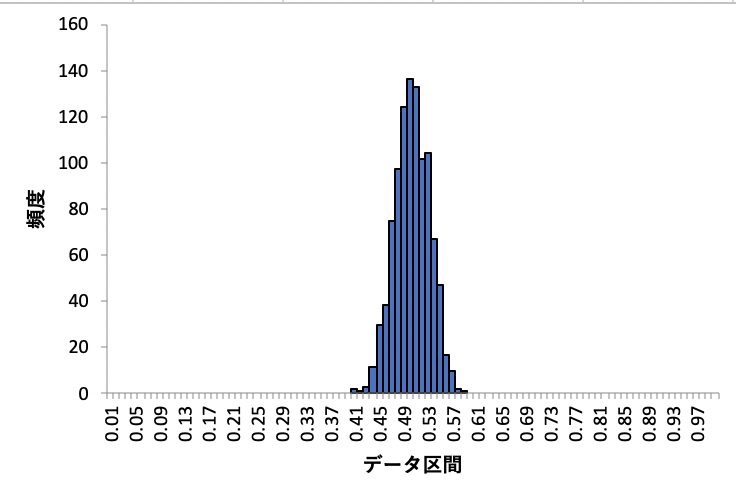
\includegraphics[scale=0.7]{kadai4_2graph5.png}
    \end{center}
    \caption{}
\end{figure}

\subsection{レポート課題}
\subsubsection*{レポート課題2-1}
\begin{shadebox}
    実験2の結果をまとめよ。
\end{shadebox}

\subsubsection*{レポート課題2-2}
\begin{shadebox}
    大数の法則とは何か、実験2の結果に基づいて説明せよ。
\end{shadebox}

\subsubsection*{レポート課題2-3}
\begin{shadebox}
    中心極限定理とは何か、実験2の結果に基づいて説明せよ。
\end{shadebox}

\subsubsection*{レポート課題2-4}
\begin{shadebox}
    区間 [0,1] の一様分布から12個選び、その合計から6を引いた値をYとする。
    Y はどのような分布に従うか述べよ。
\end{shadebox}

\section{実験3}
正規分布を基にした実験

\subsection{目標}
\begin{itemize}
    \item データを視覚的に表現する方法を理解する
    \item データの正しい要約を行う
\end{itemize}

\subsection{実験手順}
\begin{itemize}
    \item[(1)] 年収データの平均値・中央値・最頻値を求める
    \item[(2)] 年収を50万円刻みで区切ったヒストグラムを作成する
    \item[(3)] 箱ひげ図を作成する
\end{itemize}

\subsection{実験結果}
\begin{figure}[h]
    \begin{center}
        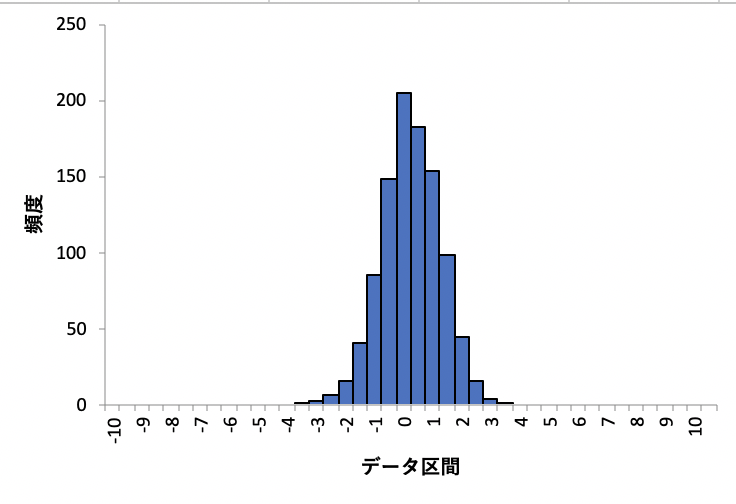
\includegraphics[scale=0.7]{kadai4_3graph1.png}
    \end{center}
    \caption{}
\end{figure}
\begin{figure}[h]
    \begin{center}
        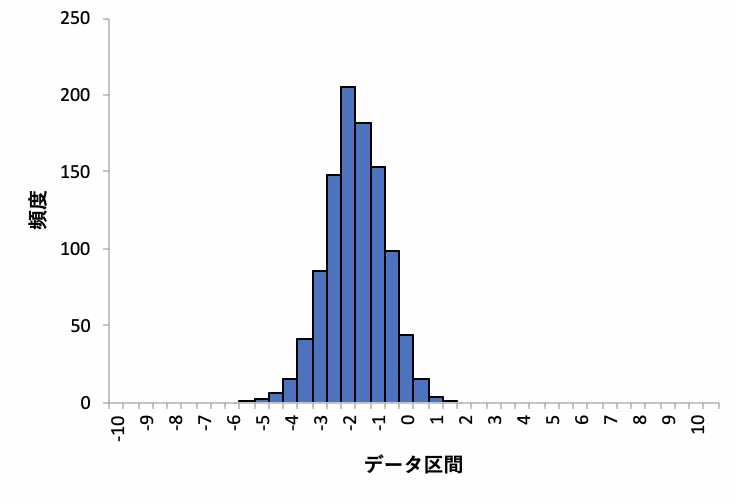
\includegraphics[scale=0.7]{kadai4_3graph2.png}
    \end{center}
    \caption{}
\end{figure}
\begin{figure}[h]
    \begin{center}
        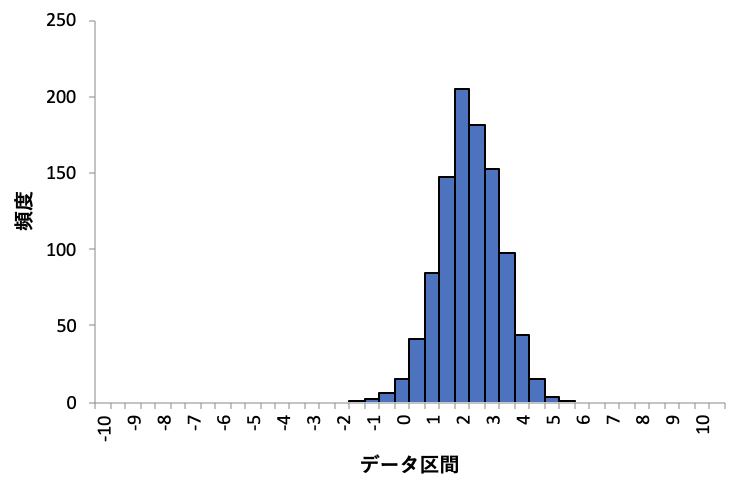
\includegraphics[scale=0.7]{kadai4_3graph3.png}
    \end{center}
    \caption{}
\end{figure}
\begin{figure}[h]
    \begin{center}
        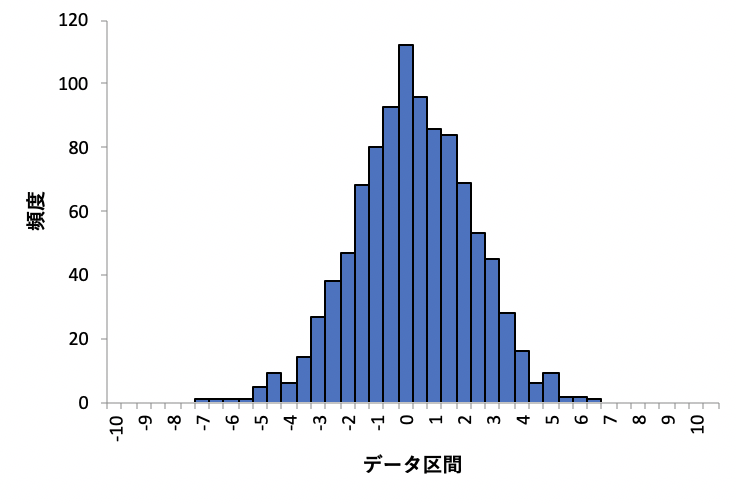
\includegraphics[scale=0.7]{kadai4_3graph4.png}
    \end{center}
    \caption{}
\end{figure}
\begin{figure}[h]
    \begin{center}
        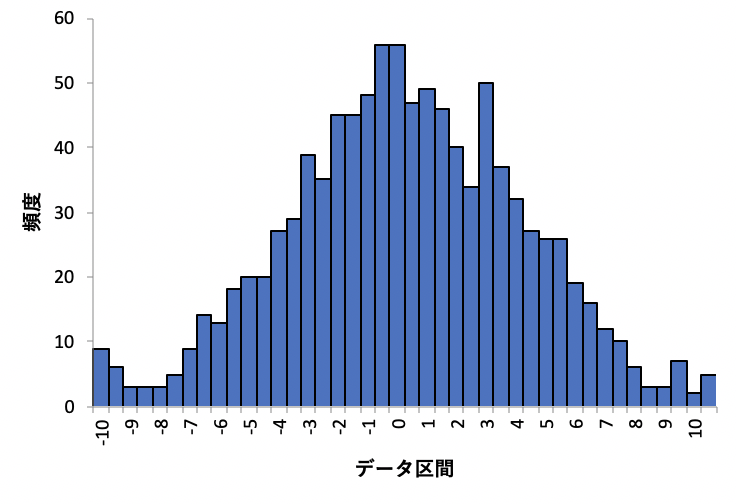
\includegraphics[scale=0.7]{kadai4_3graph5.png}
    \end{center}
    \caption{}
\end{figure}

\subsection{レポート課題}
\subsubsection*{レポート課題3-1}
\begin{shadebox}
    実験3-5、3-6で作成したヒストグラムを比較して、考察せよ。
\end{shadebox}

\subsubsection*{レポート課題3-2}
\begin{shadebox}
    実験3-5、3-7で作成したヒストグラムを比較して、考察せよ。
\end{shadebox}

\subsubsection*{レポート課題3-3}
\begin{shadebox}
    課題3-1、3-2から、
    正規分布における期待値と標準偏差は確率分布の何を決定しているといえるか述べよ。
\end{shadebox}
\subsubsection*{レポート課題3-4}
\begin{shadebox}
    偏差値の確率密度関数を書け。
\end{shadebox}
\subsubsection*{レポート課題3-5}
\begin{shadebox}
    試験の点数や順位と比較して偏差値の短所・長所を述べよ。
\end{shadebox}
\clearpage
\begin{figure}[h]
    \begin{center}
        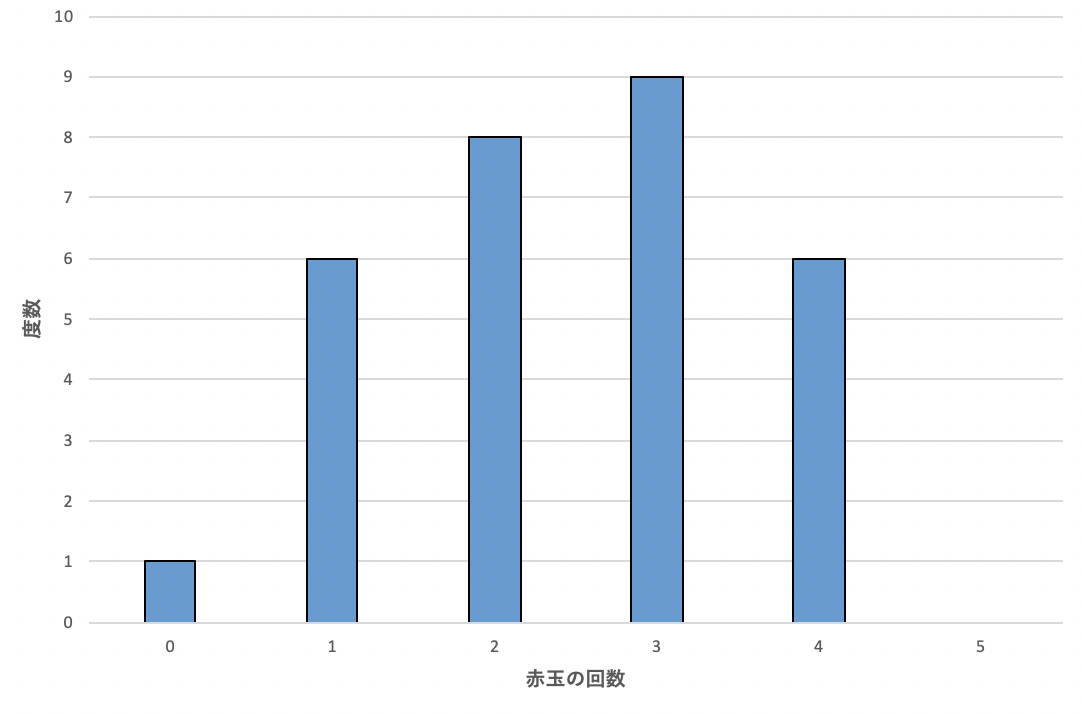
\includegraphics[scale=0.8]{kadai4_1graph1.png}
    \end{center}
    \caption{東京都の人口の推移}
    \label{fig6}
\end{figure}

表3は、文献\cite{paa}より東京都の1900年から2018年の人口を示した表である。
これをもとにグラフを作成する。
時間の推移に対して人口のデータがあるので、折れ線グラフが適切であると考えた。
したがって、図6に東京都の人口の推移を折れ線グラフで示した。

図6を見るとほとんど増加傾向であるが、1945年前後で急激に低下している。
これは、日本が戦争を行っていたので、
戦死等の理由から人口が減少したと考える。
また、2000年以降に人口増加が大きいので、
経済成長により、都市部に人口が集中していると考える。
\clearpage

\section{結論}
実験で得られたデータがばらつくことを理解した。
また、データを視覚化する方法を学び、
データの要約指標のうち代表的なものを学んだ。

\section{感想}
グラフを読み取ったり考察するのは楽しかったが、
エクセルのデータをtexの表に変換する作業がとても大変だった。
% 参考文献
\begin{thebibliography}{99}
    \label{sannkoubunnkenn_chapter}
    \bibitem[1]{rikadai}東京理科大学工学部情報工学科「情報工学実験1 2020年度」
    (2020/4/6)

    \bibitem[2]{paa}東京都統計年鑑 平成30年 | 2 人口・世帯

    \url{https://www.toukei.metro.tokyo.lg.jp/tnenkan/2018/tn18q3i002.htm}

    最終閲覧日:2020/8/3

\end{thebibliography}

\appendix
%%%%%%%%%%%%%%%%%%%%%%%%%%%%%%%%%%%%%%%%%%%%%%%%%%%%%%%
\end{document}
